
\begin{tikzpicture}[node distance=2cm, auto]
    % Nodes
    \node [draw, rectangle, minimum width=2cm, minimum height=1cm, align=center, label=above:$x(t)$, label=below:Stimulus] (stimulus) {\includegraphics[scale=0.15]{IMAGES/BACKGROUND/stim.pdf}};
    
    \node [draw, fill=blue!20, rectangle,  minimum width=11.6cm, minimum height=18cm, right=0.5cm of stimulus,  label=above:\textbf{GLM}, ] (GLM_Box) {};

    \node [draw, fill=white, rectangle,  minimum width=2.5cm, minimum height=2.5cm, right=1cm of stimulus, align=center, label=above:$k_1$, label={[align=center]below:Feedforward \\ filter}, shift={(0, 4)}] (k1) {\includegraphics[scale=0.1]{IMAGES/BACKGROUND/kfilter.pdf}};

    \node [draw, fill=white, circle, right=0.5cm of k1, align=center] (plus1) {+};

    \node [draw, fill=white, rectangle, minimum width=1cm, minimum height=1cm, above=2cm of plus1, align=center ,label={[align=center]above:Constant}] (cst1) {$C_1$};
    
    \node [draw, fill=white, rectangle,  minimum width=2.5cm, minimum height=2.5cm, right=0.5cm of plus1, align=center, label=above:$f_1$, label={[align=center]below:Nonlinear \\ function}] (f1) {\includegraphics[scale=0.1]{IMAGES/BACKGROUND/ffunction.pdf}};

    \node [draw, fill=white, rectangle,  minimum width=2.5cm, minimum height=2.5cm, right=1cm of f1, align=center, label=above:, label={[align=center]below:Probabilistic \\ process}] (Aleatoire1) {\includegraphics[scale=0.2]{IMAGES/BACKGROUND/Stocha_process.jpg}};

    \node [draw, rectangle,  minimum width=2cm, minimum height=1cm, right=1cm of Aleatoire1, align=center, label=above:$y_1(t)$, label=below:Responses ] (y1) {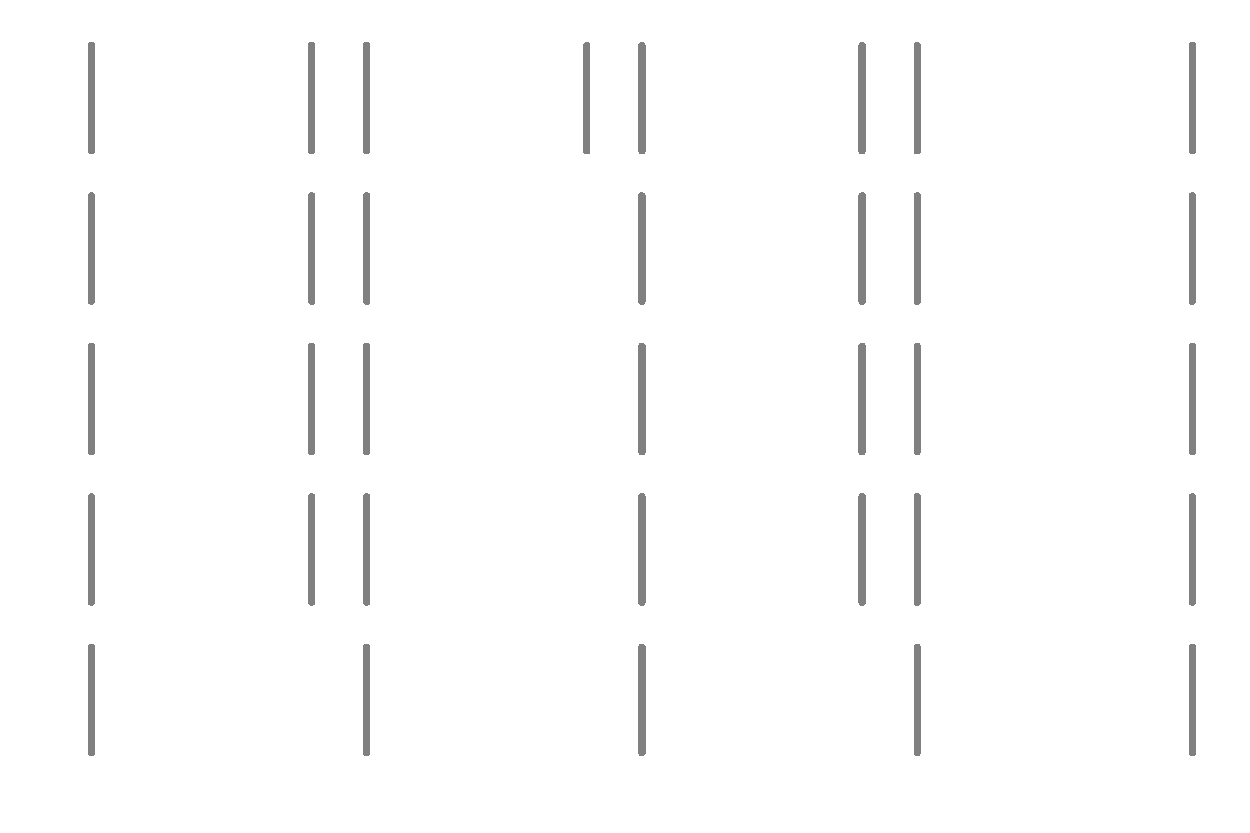
\includegraphics[scale=0.1]{IMAGES/BACKGROUND/y_out.pdf}};

    \node [draw, fill=white, rectangle,  minimum width=2cm, minimum height=1cm, right=0cm of f1, align=center, label=above:$h_{1,1}$, label={[align=center]below:Feedback \\ filter}, shift={(-0.5, 3.5)}  ] (h1) {\includegraphics[scale=0.1]{IMAGES/BACKGROUND/hfilter.pdf}};

    %--------

    \node [draw, fill=white, rectangle,  minimum width=2.5cm, minimum height=2.5cm, above=-10cm of k1, align=center, label=above:$k_2$, label={[align=center]below:Feedforward \\ filter}] (k2) {\includegraphics[scale=0.1]{IMAGES/BACKGROUND/kfilter.pdf}};

    \node [draw, fill=white, circle, right=0.5cm of k2, align=center] (plus2) {+};

    \node [draw, fill=white, rectangle, minimum width=1cm, minimum height=1cm, below=2cm of plus2, align=center ,label={[align=center]below:Constant}] (cst2) {$C_2$};
    
    \node [draw, fill=white, rectangle,  minimum width=2.5cm, minimum height=2.5cm, right=0.5cm of plus2, align=center, label=above:$f_2$, label={[align=center]below:Nonlinear \\ function}] (f2) {\includegraphics[scale=0.1]{IMAGES/BACKGROUND/ffunction.pdf}};

    \node [draw, fill=white, rectangle,  minimum width=2.5cm, minimum height=2.5cm, right=1cm of f2, align=center, label=above:, label={[align=center]below:Probabilistic \\ process}] (Aleatoire2) {\includegraphics[scale=0.2]{IMAGES/BACKGROUND/Stocha_process.jpg}};

    \node [draw, rectangle,  minimum width=2cm, minimum height=1cm, right=1cm of Aleatoire2, align=center, label=above:$y_2(t)$, label=below:Responses ] (y2) {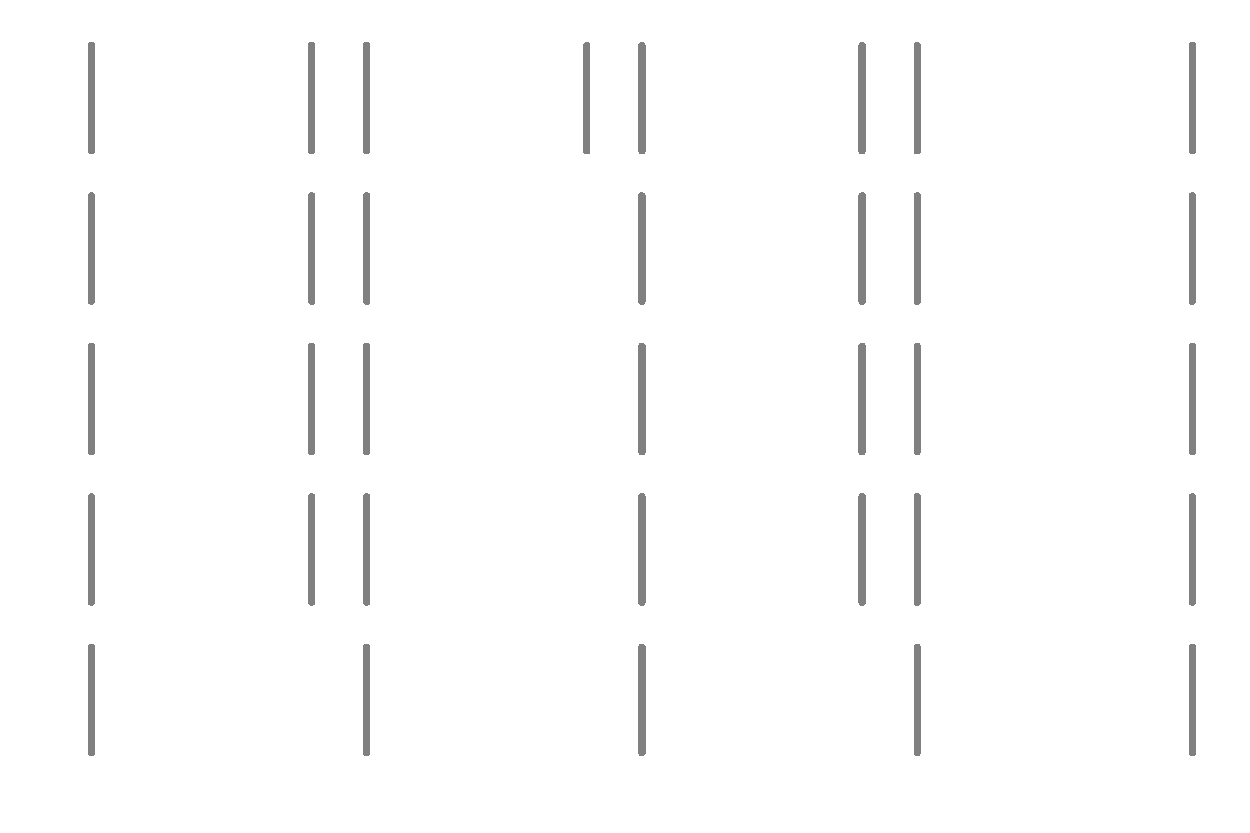
\includegraphics[scale=0.1]{IMAGES/BACKGROUND/y_out.pdf}};

    \node [draw, fill=white, rectangle,  minimum width=2cm, minimum height=1cm, right=0cm of f2, align=center, label=above:$h_{2,2}$, label={[align=center]below:Feedback \\ filter}, shift={(-0.5, -3.5)} ] (h2) {\includegraphics[scale=0.1]{IMAGES/BACKGROUND/hfilter.pdf}};


    \node [draw, fill=white, rectangle,  minimum width=2cm, minimum height=1cm, right= 0cm of f1, align=center, label=above:$h_{1,2}$, label={[align=center]below:Coupling filters}, shift={(-0.5, -3.1)} ] (c12) {\includegraphics[scale=0.1]{IMAGES/BACKGROUND/hfilter_coupled.pdf}};

    \node [draw, fill=white, rectangle,  minimum width=2cm, minimum height=1cm, above=-2.65cm of c12, align=center, label=below:$h_{2,1}$] (c21) {\includegraphics[scale=0.1]{IMAGES/BACKGROUND/hfilter_coupled.pdf}};

    % Arrows
    \draw [->] (stimulus.east) -- (k1.west);
    \draw [->] (k1) -- (plus1);
    \draw [->] (cst1) -- (plus1);
    \draw [->] (plus1) -- (f1);
    \draw [->] (f1) -- node[above] {$\lambda_1 (t)$}  (Aleatoire1);
    \draw [->] (Aleatoire1) -- (y1);
    \draw (Aleatoire1.east) edge[->, out=0, in=0,] (h1.east);
    \draw (h1.west) edge[->, out=180, in=90] (plus1.north);

    \draw [->] (stimulus.east) -- (k2.west);
    \draw [->] (k2) -- (plus2);
    \draw [->] (cst2) -- (plus2);
    \draw [->] (plus2) -- (f2);
    \draw [->] (f2) -- node[above] {$\lambda_2 (t)$}  (Aleatoire2);
    \draw [->] (Aleatoire2) -- (y2);
    \draw (Aleatoire2.east) edge[->, out=0, in=0,] (h2.east);
    \draw (h2.west) edge[->, out=180, in=270] (plus2.south);


        \draw (Aleatoire1.east) edge[->, out=0, in=0] (c12.east);
        \draw (Aleatoire2.east) edge[->, out=0, in=0] (c21.east);
        
        \draw (c12.west) edge[->,out=180, in=90] (plus2.north);
        \draw (c21.west) edge[->,out=180, in=270] (plus1.south);



  
\end{tikzpicture}